\def\pgfsysdriver{pgfsys-dvisvgm.def}
% flashcards-title: Reinforcing and counteracting feedback loops
% flashcards-desc: Two three-component loops use text labels on arrows. Panel A has three increase links. Panel B has two increase links and one decrease link; no feedback category is named.
\documentclass[tikz,border=6pt]{standalone}
\usetikzlibrary{arrows.meta,calc,fit,positioning,shapes.geometric}

\definecolor{fcink}{HTML}{17212B}
\definecolor{fcblue}{HTML}{1D5D8C}
\definecolor{fcgreen}{HTML}{2D6A4F}
\definecolor{fcorange}{HTML}{A44A1F}
\definecolor{fcpale}{HTML}{F4F7F9}
\definecolor{fcsoil}{HTML}{8B5E3C}

\tikzset{
  fc text/.style={font=\sffamily, text=fcink},
  fc panel/.style={draw=fcink, line width=0.9pt, rounded corners=5pt, fill=fcpale},
  fc node/.style={draw=fcink, line width=0.9pt, rounded corners=4pt, fill=white,
    minimum width=24mm, minimum height=10mm, align=center, font=\sffamily},
  fc arrow/.style={-{Stealth[length=3.2mm,width=2.4mm]}, line width=1.2pt,
    draw=fcblue, line cap=butt},
  fc boundary/.style={draw=fcorange, line width=1.4pt, dash pattern=on 5pt off 3pt,
    rounded corners=7pt},
  fc label/.style={font=\sffamily\bfseries, text=fcink},
  fc note/.style={font=\sffamily\small, text=fcink, align=center}
}

\begin{document}
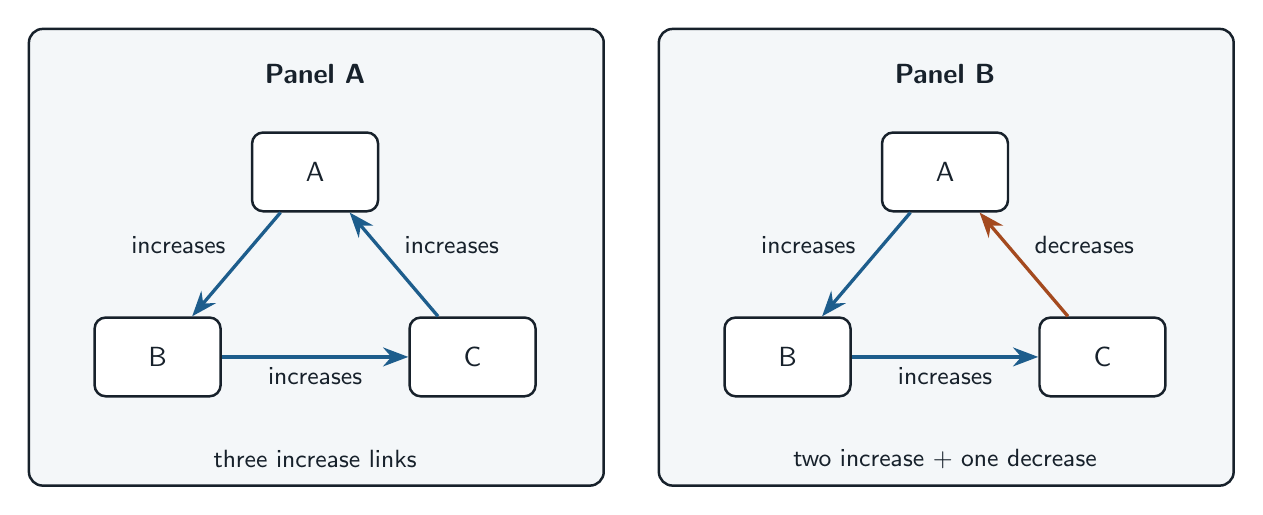
\begin{tikzpicture}[fc text, x=1cm, y=1cm]
  \node[fc panel, minimum width=73mm, minimum height=58mm, anchor=south west] at (0,0) {};
  \node[fc panel, minimum width=73mm, minimum height=58mm, anchor=south west] at (8.0,0) {};
  \node[fc label] at (3.65,5.25) {Panel A};
  \node[fc label] at (11.65,5.25) {Panel B};
  \foreach \o in {0,8} {
    \node[fc node, minimum width=16mm] (a\o) at (\o+3.65,4.0) {A};
    \node[fc node, minimum width=16mm] (b\o) at (\o+1.65,1.65) {B};
    \node[fc node, minimum width=16mm] (c\o) at (\o+5.65,1.65) {C};
    \draw[fc arrow] (a\o)--node[fc note, above left] {increases} (b\o);
    \draw[fc arrow] (b\o)--node[fc note, below] {increases} (c\o);
  }
  \draw[fc arrow] (c0)--node[fc note, above right] {increases} (a0);
  \draw[fc arrow, draw=fcorange] (c8)--node[fc note, above right] {decreases} (a8);
  \node[fc note] at (3.65,0.35) {three increase links};
  \node[fc note] at (11.65,0.35) {two increase + one decrease};
\end{tikzpicture}
\end{document}
